% This is file JFM2esam.tex
% fieserachst release v1.0, 20th October 1996
%       release v1.01, 29th October 1996
%       release v1.1, 25th June 1997
%       release v2.0, 27th July 2004
%       release v3.0, 16th July 2014
%   (baseue on JFMsampl.tex v1.3 for LaTeX2.09)
% Copyright (C) 1996, 1997, 2014 Cambridge University Press

\documentclass{jfm}
\usepackage{graphicx}
\usepackage{mathtools}
\usepackage{epstopdf, epsfig}
\usepackage{tikz}
\usepackage[ruled]{algorithm2e}
\usepackage{booktabs}
\usepackage{array}
\usepackage{amsmath}
\usepackage{multirow}
\usepackage{comment}
\usepackage{natbib}
\usepackage{nomencl}
\usepackage[]{color}
\usepackage[]{xcolor}
\usepackage{todonotes}
\usepackage{placeins}
\usepackage{relsize}
\usepackage{soul}
\usepackage{comment}
\usepackage{listings}
\usepackage[tikz]{bclogo}
\usepackage{tikz}
\usepackage{ulem}
\usetikzlibrary{patterns}
\usepackage{cancel}




\usepackage[most,skins,theorems]{tcolorbox}
\newtcolorbox[blend into=figures]{myfigure}[2][label=<>,colback=blue!5,colframe=blue!75,boxsep=2mm,left=0mm,right=0mm, top=0mm, bottom=0mm]{float=htb, title={#2}, #1}
\addtolength{\textfloatsep}{-14pt}
\presetkeys{bclogo}{
ombre=true,
epBord=1,
couleur = blue!2!white,
couleurBord = gray,
arrondi = 0.1,
logo=\bcoutil
}{}
\usepackage{color} %red, green, blue, yellow, cyan, magenta, black, white
\definecolor{mygreen}{RGB}{28,172,0} % color values Red, Green, Blue
\definecolor{mylilas}{RGB}{170,55,241}
\lstset{language=Matlab,%
    %basicstyle=\color{red},
    breaklines=true,%
    morekeywords={matlab2tikz},
    keywordstyle=\color{blue},%
    morekeywords=[2]{1}, keywordstyle=[2]{\color{black}},
    identifierstyle=\color{black},%
    stringstyle=\color{mylilas},
    commentstyle=\color{mygreen},%
    showstringspaces=false,%without this there will be a symbol in the places where there is a space
    %numbers=left,%
    %numberstyle={\tiny \color{black}},% size of the numbers
    %numbersep=9pt, % this defines how far the numbers are from the text
    emph=[1]{for,end,break},emphstyle=[1]\color{red}, %some words to emphasise
    %emph=[2]{word1,word2}, emphstyle=[2]{style},    
}

\tcbset{highlight math style={enhanced,
  colframe=red,colback=white,arc=0pt,boxrule=1pt}}
  
%\newcommand*{\transpose}{{\!\!\scriptscriptstyle{\mathrm{T}}}}
\newcommand*{\boxcolor}{orange}
\makeatletter
\newcommand{\crossedout}[2]{\textcolor{\boxcolor}{%
\tikz[baseline={([yshift=-0.5ex]current bounding box.center)}] \node(#2) [opacity=0,text opacity=1,pattern color=red!50!white,pattern=north west lines,rectangle,inner sep=1pt,rounded corners] {\normalcolor\m@th$\displaystyle#1$};}}
 \makeatother

\makeatletter
\newcommand{\boxedeqn}[2]{\textcolor{\boxcolor}{%
\tikz[baseline={([yshift=-0.5ex]current bounding box.center)}] \node(#2) [opacity=0,text opacity=1,red,inner sep=1pt,rounded corners,draw] {\normalcolor\m@th$\displaystyle#1$};}}
 \makeatother

% Designate a term in a math environment to point to
% Syntax: \mathterm[node label]{some math}
\newcommand\mathterm[2][]{%
   \tikz [baseline] { \node [mathterm] (#1) {$#2$}; }}


\usepackage{tcolorbox}
\newcolumntype{x}[1]{>{\centering\arraybackslash\hspace{0pt}}p{#1}}

\newcommand{\centered}[1]{\begin{tabular}{l} #1 \end{tabular}}

\newtheorem{lemma}{Lemma}
\newtheorem{corollary}{Corollary}

\SetKwInput{KwInput}{Input}                % Set the Input
\SetKwInput{KwOutput}{Output}              % set the Output

%commands used for equations
\newcommand\norm[1]{\left\lVert#1\right\rVert}
\newcommand{\solution}{\mathbf{q}}
\newcommand{\transpose}{\mathrm{T}}
\newcommand{\cntrVec}{\mathbf{c}}
\newcommand{\cntrVecMember}[1]{\mathbf{c}^{(#1)}}
\newcommand{\cost}{\mathcal{J}}
%\newcommand{\cost}{{J}}
\newcommand{\meas}{\mathbf{m}}
\newcommand{\projCntrVec}{\mathcal{M}(\solution)}
\newcommand{\projCntrVecMean}{\mathcal{M}(\solution_i)}
\newcommand\projCntrVecEns[1]{\mathcal{M}(\solution^{\scriptscriptstyle{(#1)}})}
\newcommand{\covCntrVec}{\Sigma_\mathbf{c}}
\newcommand{\covMeasVec}{\Sigma_\mathbf{m}}
\newcommand{\Weight}{\mathbf{W}_{\!s}}
\newcommand{\pertMat}{\mathbf{P}}
\newcommand{\obsMat}{\mathbf{H}}
\newcommand{\hessian}{\mathcal{H}}
\newcommand{\gradLogLiklihood}{\mathbf{g}}
\newcommand{\weights}{\mathbf{w}}
\newcommand{\Nens}{{N}}
\newcommand{\expectation}{\mathbb{E}}
\newcommand{\identity}{\mathbf{I}}
\newcommand{\AMat}{\mathbf{A}}
\newcommand{\BMat}{\mathbf{B}}
\newcommand{\imag}{\mathrm{i}}

%Time horizon and frequency of acquitiion
\newcommand{\measHorizon}{T_{a}}
\newcommand{\measFrequency}{\Delta t_a}

%Linearization of cost
\newcommand{\LinCost}{\widetilde{\cost}}

%---------- End of definition of line types ------
\setlength{\marginparwidth}{1.5cm}
\def\del#1{\textcolor{gray}{#1}}
\def\delmargin#1{\todo[color=gray!40,size=\tiny]{#1}}
%
\def\jy#1{\textcolor{Green}{#1}}
\def\jymargin#1{\todo[color=Green!40,size=\tiny]{#1}}
%
\def\tz#1{\textcolor{blue}{#1}}
\def\tzmargin#1{\todo[color=blue!20,size=\tiny]{#1}}
%
\def\db#1{\textcolor{red}{#1}}
\def\dbmargin#1{\todo[color=red!40,size=\tiny]{#1}}
%
% \def\outline#1{\textcolor{Gray}{#1}}
% \def\outline#1{\textcolor{Gray}{}}
\allowdisplaybreaks[1]
%--------------------------------------------------------

\title{Adjoint-based sensitivity using DGM}
\author{David A. Buchta}
\begin{document}

\maketitle

%highlight mesh free; trained on batches of randomly sampled points; 
\begin{abstract}
 The adjoint state is useful for optimization, sensitivity analysis, data assimilation, experimental design, etc. However, acquiring the solution is costly, since it often requires access to the entire trajectory of the forward state. Practioners cope with this challenge in several ways: i) recomputing the forward state when needed, ii) storing the forward trajectory in memory, or iii) a mixture of these. To mitigate these complications, the forward and adjoint solutions are approximated using the Deep Galerkin Method~\citep{sirignano2018dgm}. The neural-network weights, for each network, minimize the residual of the forward and adjoint PDEs and their boundary conditions. We demonstrate the approach on an advection-diffusion equation, where the objective is to identify the sensitivity of the solution to initial-condition perturbations.  Gradient accuracy for adjoint-forward DGM is compared with standard discretization methods, e.g., finite-difference techniques. 
\end{abstract}

\vspace{-24pt}\makenomenclature
\nomenclature[01]{$\mathcal{J}$}{`engineering' objective function}
\nomenclature[02]{$\mathcal{L}$}{neural network objective function}
\nomenclature[03]{$u$}{forward state}
\nomenclature[04]{$u^\dagger$}{adjoint state}
\nomenclature[05]{$f$}{neural network approximation of forward state}
\nomenclature[06]{$f^\dagger$}{neural network approximation of forward state}
%\nomenclature{$\mathcal{V}$}{spatial domain volume}
%\nomenclature{$\mathcal{T}$}{temporal domain}
\nomenclature[07]{$\mathcal{M}$}{forward conservation equations}
\nomenclature[08]{$\mathcal{M}^\dagger$}{adjoint equations}
\nomenclature[09]{$\theta$}{forward neural network weights}
\nomenclature[09]{$\theta^\dagger$}{adjoint neural network weights}
\nomenclature[10]{$||\cdot||$}{L2 norm}
\printnomenclature
\vspace{-6pt}

\section{Adjoint-Forward Deep Galerkin Method (AFDGM)}
Consider the scalar cost function
\begin{equation}\label{eq:genCost}
    \mathcal{J}(u) = \frac{1}{2} \int_\mathcal{T} \int_\Omega I(u(x,T))\,d\Omega d\mathcal{T},
\end{equation}
where the solution at the end of the time period of interest, $u(x,T)$, is acquired by solving the following PDE system
\begin{align}\noindent 
    \mathcal{M}(u) \equiv \partial_t u(x,t) + \mathcal{D}(u) u(x,t) &= 0 \quad (x,t) \in \mathcal{T}\times \Omega\\
    u(x,t=0)&=u_0(x)\\
    u(x,t)&=b(x,t)\quad x \in \partial\Omega.
\end{align}
The operator $\mathcal{D}(u)$ is potentially nonlinear; $u_0(x)$ is the initial conditions; and, $b(x,t)$ are the boundary conditions.
The objective is to identify earlier state perturbations $\delta u(x,t)$ for $t<T$ that optimizes the cost in (\ref{eq:genCost}), e.g., initial condition perturbations that increase (or decrease) the cost. One approach is to use the local gradient of the cost to guide the direction of increase, $\delta u(x,t=0)=\beta \nabla \mathcal{J}$. The gradient is obtained by considering the first-order variation of $\mathcal{J}$ and subtracting the constraint of that perturbations of the state $\delta u(x,t)$ must obey the PDE system,
\begin{equation}
    \delta \mathcal{J}(u) = \partial_u \mathcal{J} \delta u - \int_\mathcal{T} \int_\Omega (u^\dagger \partial \mathcal{M}_u \delta u )\,d\Omega d\mathcal{T}. \end{equation}
Substituting the PDE, the change in the cost is
\begin{equation}
    \delta \mathcal{J}(u) = \int_\Omega \partial_u I(u) \delta u(x,T)\,d\Omega - \int_\mathcal{T} \int_\Omega u^\dagger\left[\partial_t \delta u(x,t) + \partial_u\mathcal{D}\delta u(x,t) \right]\,d\Omega d\mathcal{T},
\end{equation}
and integrating by parts
\begin{align}\label{eq:expandedVarJ}
    \delta \mathcal{J}(u) &=\int_\Omega u^\dagger(x,0)\delta u(x,0)\,d\Omega\\\nonumber &+\int_\Omega \partial_u I(u) \delta u(x,T)-u^\dagger(x,T)\delta u(x,T)\,d\Omega \\\nonumber
    &- \int_\mathcal{T} \int_\Omega \delta u\left[\partial_t  u^\dagger(x,t) + \mathcal{D}^\dagger(u)u^\dagger(x,t) \right]\,d\Omega d\mathcal{T} - B(u^\dagger,\delta u),
\end{align}
where $B(u^\dagger,\delta u)$ represent spatial boundary terms which depend on the form of $\mathcal{D}$, isolates state perturbations $\delta u$ from within the evolution of the PDE. 
The following adjoint PDE system 
\begin{align}\noindent \label{eq:adjoint}
    \mathcal{M}^\dagger(u,u^\dagger) \equiv \partial_t u^\dagger(x,t) + \mathcal{D}^\dagger(u) u^\dagger(x,t) &= 0 \quad (x,t) \in \mathcal{T}\times \Omega\\
    u^\dagger(x,T)&=\partial_u I(u(x,T))\\\label{eq:adjbc}
    u^\dagger(x,t)&=b^\dagger(x,t)\quad x \in \Omega
\end{align}
is judiciously chosen such the last two lines in (\ref{eq:expandedVarJ}) are zero, which furnishes a direct relationship between initial condition perturbations $\delta u(x,0)$ and changes in the cost function $\delta \mathcal{J}$ via
\begin{equation}\nonumber
    \delta \mathcal{J}(u) =\int_\Omega u^\dagger(x,0)\delta u(x,0)\,d\Omega.\\
\end{equation}
Solving (\ref{eq:adjoint}-\ref{eq:adjbc}) for $u^\dagger$, the change in cost $\delta \mathcal{J}$ can be found for \textit{any} initial condition perturbation. However, the expression depends on evolving the adjoint solution from time $t=T$ to $t=0$, which in general depends on the entire state of $u(x,t)$ via $\mathcal{D}^\dagger(u)$ in (\ref{eq:adjoint}).  For practical applications, accessing $u(x,t)$ can be onerous in terms of memory and computational expense (see \cite{vishnampet2015practical} for example and discussion), making low-cost low-memory approximations of $u$ (and $u^\dagger$) attractive. Thus, the adjoint-forward deep Galerkin method (AFDGM) approximates both $u$ and $u^\dagger$ with deep neural networks $f(x,t; \theta)$ and $f^\dagger(x,t; \theta^\dagger)$. The parameters of the neural networks $\Theta=\left\{\theta,\theta^\dagger \right\}$ are found by minimizing 
\begin{align}\label{eq:loss}\mathcal{L}(f,f^\dagger) &= \underbrace{||\mathcal{M}(f)||^2}_{\mathcal{L}_{PDE}} + \underbrace{||f(\cdot,0)-u_0||^2}_{\mathcal{L}_{IC}} + \underbrace{||f(\hat{x},t)-b(\hat{x},t)||^2}_{\mathcal{L}_{BC}}\\ 
    &+\underbrace{||\mathcal{M}^\dagger(f,f^\dagger)||^2}_{\mathcal{L}^\dagger_{PDE}} + \underbrace{||f^\dagger(\cdot,T)-\partial_f I(f(x,T))||^2}_{\mathcal{L}^\dagger_{IC}} + \underbrace{||f^\dagger(\hat{x},t)-b^\dagger(\hat{x},t)||^2}_{\mathcal{L}^\dagger_{BC}}\nonumber
    \end{align}
where $\hat{x} \in \partial \Omega$.
Note the explicit coupling between the approximate forward and adjoint solutions when terms in the PDE and initial conditions are evaluated. The AFDGM algorithm, which is an adaptation of DGM~\citep{sirignano2018dgm}, is provided in Algorithm~\ref{alg:afdgm}. An example of the evolution of the loss function and component terms of (\ref{eq:loss}) is show in figure~\ref{fig:evolutionLoss}.  Notice, similar trends in $\mathcal{L}_{PDE}$ and $\mathcal{L}^\dagger_{IC}$, which shows the coupling between the two neural network models: as $u$ and $u(x,T)$ converges to the true solution so does the initial condition of the adjoint which depends on the forward state $u^\dagger(x,T)=\partial_u I(u(x,T))$.  The following section provides an example of AFDGM applied to the advection-diffusion equation.

\begin{figure}
    \centering
    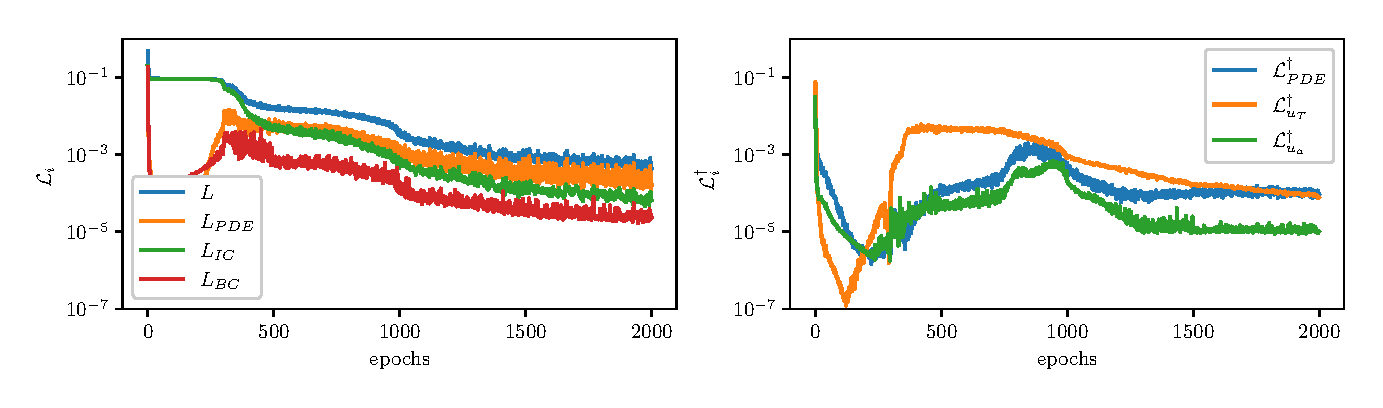
\includegraphics[width=\textwidth]{./figures/dgmaf_loss_functions.eps}
    \caption{Evolution of the loss function components.}
    \label{fig:evolutionLoss}
    \vspace*{6pt}
\end{figure}


\begin{minipage}{1\textwidth}
\begin{algorithm}[H]
\SetAlgoLined
%\begin{itemize}
\KwInput{Number of sampled points in the domain $N$}

Initialize the optimizer learning rate $r$\\
Initialize neural network parameters, $\Theta=\left\{\theta,\theta^\dagger \right\}$, using the Xavier method\\
$j=0$\\
 \While{Insufficient reduction in objective function}{
  Generate $N$ random samples $s_n=\{x_n, t_n\}$ in the spatial/temporal domain \\
  \For{$N_b$ number of iterations per batch}
{
  Construct the forward-adjoint objective function $\mathcal{L}=\mathcal{L}_{PDE}+\mathcal{L}_{BC}+\mathcal{L}_{IC}+\mathcal{L}^\dagger_{PDE}+\mathcal{L}^\dagger_{BC}+\mathcal{L}^\dagger_{TC}$\\
  Update $\Theta=\left\{\theta,\theta^\dagger \right\}$ with stochastic gradient descent step\\\hspace{12pt}$\Theta_{j+1}=\Theta_j - r \nabla_\Theta \mathcal{L}(\Theta)$\\
  $j\leftarrow j+1$
  }
  Update learning rate $r$ according to prescribed schedule, e.g., $r\leftarrow r/10^n$\\
  %$i\leftarrow i+1$
 }
 \KwResult{Forward and adjoint neural networks: $f(x,t,\mathbf{p};\theta)$ and $f^\dagger(x,t,\mathbf{p};\theta^\dagger)$}
\caption{Algorithm for AFDGM}
 \label{alg:afdgm}
\end{algorithm}
\end{minipage}

\section{Sensitivity in the advection-diffusion equation}
The approach described in the previous section is applied in the context of the linear advection-diffusion system. The objective is to determine what initial condition perturbations $\delta u(x,0)$ increase the final state energy
\begin{equation}
    \mathcal{J}(u) = \frac{1}{2} \int_\Omega u(x,T)^2\,d\Omega.
\end{equation}
The forward system is
\begin{align}
    \frac{\partial u}{\partial t} + c \frac{\partial u}{\partial x} - \nu \frac{\partial^2 u}{\partial x^2} = 0 \\
    u(x,t=0)=f(x) \quad x \in \Omega,
\end{align}
where the advection speed is $c=1.0$ and the diffusion coefficient is $\nu=0.01$. The initial condition is $f(x)=\exp\left[-(x-0.5)^2/0.01^2 \right]$.  The corresponding adjoint system is
\begin{align}
    \frac{\partial u^\dagger}{\partial t} + c \frac{\partial u^\dagger}{\partial x} + \nu \frac{\partial^2 u^\dagger}{\partial x^2} = 0 \\
    u^\dagger(x,t=T)=u(x,t=T) \quad x \in \Omega.
\end{align}
The boundaries are periodic, e.g. $u(0,t)=u(1,t)$, $\partial_x u(0,t)=\partial_x u(1,t)$, etc. The behavior of the forward and adjoint solutions are shown in figure~\ref{fig:evolution}(a,b). The orientation of the contours show that the advection speed is unity.  The diffusion term causes the initial Gaussian profile to spread as time advances.  The adjoint field, starting from the diffused $u(x,T)$ profile retreats from $t=T$ to $t=0$ and diffuses further.  The final profile in $u^\dagger(x,0)$ shows how to perturb the initial condition $u(x,0)$ in order to increase or decrease $\mathcal{J}$. 

The outcomes of two methods are contrasted in figure~\ref{fig:evolution}.  Gray contour lines solve the forward and adjoint methods using standard finite difference approachs: fourth-order Runge--Kutta time-discretiztaion and second-order central spatial differences.  Black contour lines represent the deep network approximations using AFDGM.   Slight discrepancies remain due to early stopping of optimizing the neural network parameters, see figure~\ref{fig:evolutionLoss}. The following section quantifies the accuracy of a cost function $\nabla \mathcal{J}$ for the deep network approximations.

\begin{figure}
    \centering
    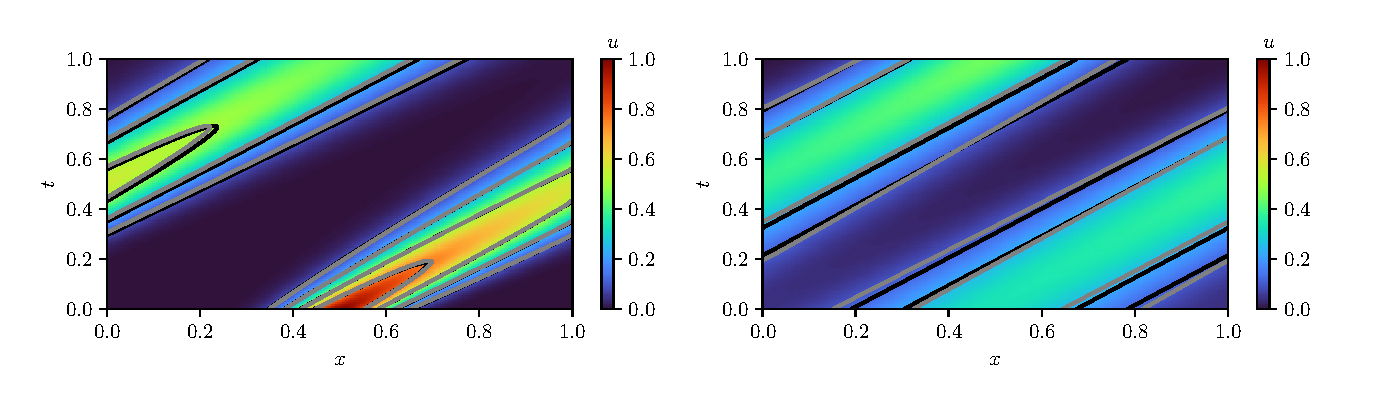
\includegraphics[width=1\textwidth]{./figures/dgmaf_space_time_solutions_overlay.eps}
    \caption{Neural network approximation of (a) $u(x,t)$ and (b) $u^\dagger(x,t)$. Colour is $f,f^\dagger$. Contour lines are $\{u,u^\dagger\}=[0.1, 0.25, 0.5 0.75]$: neural network approximations (black lines) and finite difference discretization (grey lines)}.
    \label{fig:evolution}
\end{figure}

\subsection{Assessment of accuracy}
%The selected `initial' condition of the adjoint field implies that the change in the cost function $\delta \mathcal{J} = u^\dagger(x,t=0)^\top u(x,t=0)$.  
Often, the accuracy of the gradient is assessed by using Taylor series approximation~\citep{vishnampet2015practical,buchta2016discrete}
\begin{equation}
    \mathcal{J}(u+\delta u) - \mathcal{J}(u) = \frac{\partial \mathcal{J}}{\partial u} \delta u + O(||\delta u||^2).
\end{equation}
Provided a perturbation $\delta u$, the change in the cost can be evaluated $\mathcal{J}(u_0+\delta u)-\mathcal{J}(u_0)$ by a `brute-force' manner either using standard discretization schemes or with a neural network approximation of the solution. We select perturbations of the initial condition to be in the direction of the adjoint field, $\delta u_0=\alpha u_0^\dagger$ where $\alpha > 0$ increases $\mathcal{J}$ and vice versa. The gradient error between the brute-force approach and the adjoint method is
\begin{equation}
    \varepsilon = \left|\frac{\mathcal{J}(u_0+\alpha u_0^\dagger)-\mathcal{J}(u_0)}{\alpha} - {u_0^\dagger}^\top u_0^\dagger\right| + O(\alpha),
\end{equation}
which converges at a rate $\alpha$. For $|\alpha| \ll 1$, the finite difference $\mathcal{J}(u_0+\delta u)-\mathcal{J}(u_0)$ is susceptible to numerical round-off and $\epsilon$ will increase.  Also, when $u$ and $u^\dagger$ are approximated with finite differences from the continuous PDEs, discretization errors impede convergence rates (see \cite{vishnampet2015practical}). %And, when $u^\dagger$ is approximated from the discretized PDE, convergence is only susceptible to numerical round off. 
For neural-network approximated forward and adjoint solutions, two errors are assessed:
\begin{align}
    i) &\quad \widetilde{\varepsilon} \,\,\,= \left|\frac{{\mathcal{J}}\left(u_0+\alpha u_0^\dagger\right)-{\mathcal{J}}(u_0)}{\alpha} - {{{{f^\dagger_0}}}}^\top {{f^\dagger_0}}\right| + O(\alpha)\quad \text{and}\\
    ii) &\quad \widetilde{\varepsilon}^\star = \left|\frac{{\mathcal{J}}\left(f(\alpha f_0^\dagger) \right)-{\mathcal{J}}(f)}{\alpha} - {{{{f^\dagger_0}}}}^\top {{f^\dagger_0}}\right| + O(\alpha).
\end{align}
The $\widetilde{\epsilon}$ compares the neural network gradient to the standard discretization brute-force approach; and, $\widetilde{\epsilon}^\star$ compares the neural network gradient with the forward neural network using a perturbed initial condition $f(\alpha f_0^\dagger)$. Figure~\ref{fig:accuracy} shows the relative error.
 $\varepsilon$ is the baseline we expect from solving the discretized forward and adjoint equations with standard discretization schemes. The gradient from the adjoint neural network also shows good agreement with discretized approach. However, when the neural network is used to provide $f(\alpha f_0^\dagger)$, the error is elevated. Comparing $\widetilde{\epsilon}$ and $\widetilde{\epsilon}^\star$, the elevated error is due to computing $f(\alpha f_0^\dagger)$  since the forward network was not trained on perturbations to the initial condition. Thus, the accuracy degrades. The error is further exacerbated by single precision data types used in the training which causes machine round-off to dominate by $\alpha\lesssim 10^{-1}$. In addition, nonlinearity in the neural network is apparent. For $\alpha > 1$, $\widetilde{\epsilon}^\star$ is not $\propto \alpha$.
 %Besides error magnitude, the direction of the gradient is important. The discrepancy in the angle between the neural network and standard discretization,
%\begin{equation}
%    \varphi=\cos^{-1} \frac{{f_0^\dagger}^\top u_0^\dagger}{\sqrt{||f^\dagger_0||^2 || u^\dagger_0||^2}},
%\end{equation}
%is $\varphi\approx 10^{\circ}$.  We expect that higher accuracy can be attained by enhancements to the neural network. 


\begin{figure}
    \centering
    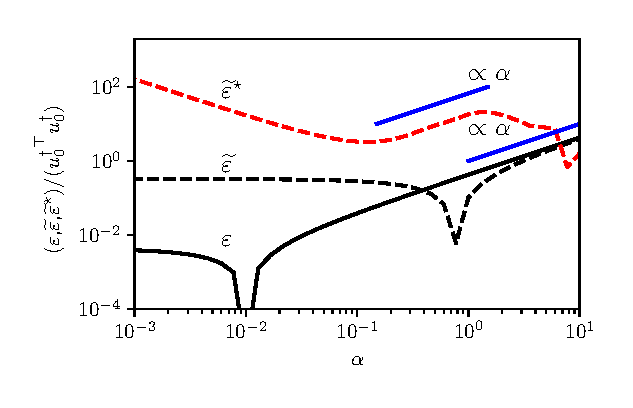
\includegraphics[width=0.655\textwidth]{./figures/dgmaf_accuracy.eps}
    \caption{Gradient accuracy assessed by perturbing the initial condition with $\delta u_0=\alpha u^\dagger$.}
    \label{fig:accuracy}
    \vspace*{12pt}
\end{figure}

\section{Discussion}
Deep learning algorithms provide efficient access to field sensitivity. Gradient accuracy shows an expected rate of convergence, and we expect that more training or deeper networks (more layers and more nodes) can enhance accuracy to a desired level.

%\appendix{Details on training}
%\begin{figure}
%    \centering
    %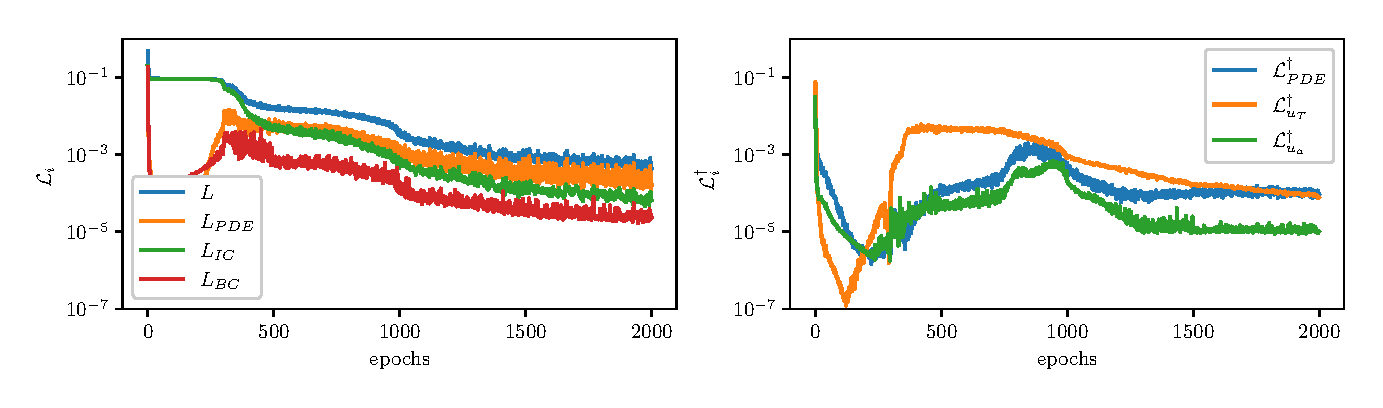
\includegraphics[width=\textwidth]{./figures/dgmaf_loss_functions.eps}
    %\caption{Evolution of the loss function components.}
    %\label{fig:my_label}
%\end{figure}

\bibliography{references}
\bibliographystyle{jfm}


\end{document}
